
\documentclass{beamer}
\setbeamertemplate{footline}[frame number]
%\usepackage{beamerthemeBerkeley}
\usetheme{Montpellier}
%\usetheme{Warsaw}
%\usetheme{Boadilla}
\usepackage[english]{babel}
\usepackage{graphicx}
%\usepackage{ams}
%\usepackage{blue}
\usepackage{amsmath} 
\usepackage{xcolor}


\newcommand{\myp}{\ensuremath{\mathbb{P}}}
\newcommand{\mye}{\ensuremath{\mathbb{E}}}
\newcommand{\myvar}{\mathbf{Var}}
\newcommand{\mycov}{\mathbf{Cov}}
\newcommand{\myind}{\ensuremath{\mathbbm{1}}}

\newcommand{\mI}{\ensuremath{\pmb{\mathsf{I}}}}
\newcommand{\mL}{\ensuremath{\pmb{\mathsf{L}}}}
\newcommand{\mQ}{\ensuremath{\pmb{\mathsf{Q}}}}
\newcommand{\mV}{\ensuremath{\pmb{\mathsf{V}}}}
\newcommand{\mW}{\ensuremath{\pmb{\mathsf{W}}}}
\newcommand{\mX}{\ensuremath{\pmb{\mathsf{X}}}}
\newcommand{\mZ}{\ensuremath{\pmb{\mathsf{Z}}}}

\newcommand{\ba}{\mathbf{a}}
\newcommand{\bd}{\mathbf{d}}
\newcommand{\bg}{\mathbf{g}}
\newcommand{\bV}{\mathbf{V}}
\newcommand{\bX}{\mathbf{X}}
\newcommand{\bY}{\mathbf{Y}}
\newcommand{\bZ}{\mathbf{Z}}

\newcommand{\bzero}{\mathbf{0}}

\newcommand{\balpha}{\mbox{\boldmath$\alpha$}}
\newcommand{\bbeta}{\mbox{\boldmath$\beta$}}
\newcommand{\bepsilon}{\mbox{\boldmath$\epsilon$}}
\newcommand{\bgamma}{\mbox{\boldmath$\gamma$}}
\newcommand{\bDelta}{\mbox{\boldmath$\Delta$}}
\newcommand{\bPhi}{\mbox{\boldmath$\Phi$}}
\newcommand{\bPsi}{\mbox{\boldmath$\Psi$}}
\newcommand{\bSigma}{\mbox{\boldmath$\Sigma$}}
\newcommand{\bmu}{\mbox{\boldmath$\mu$}}



\title{Lecture 3: GWAS in Samples with Structure \& Introduction to the REGENIE Software}

\author{Instructors: Joelle Mbatchou and Loic Yengo} 


\date{}


\begin{document}


	\begin{frame}
	\titlepage
	\vspace{-2cm}
	\begin{center}
		
		{ \Large Summer Institute in Statistical Genetics 2022\\}
		
		
	\end{center}
\end{frame}



\begin{frame}
\frametitle{\bf Introduction}
\begin{itemize}
\item Genetic association studies are widely used for the identification of genes that influence complex traits. 
\item To date, hundreds of thousands of individuals have been included in genome-wide association studies (GWAS) for the mapping of both dichotomous and quantitative traits.
\item Large-scale genomic studies often have high-dimensional data consisting of 
\begin{itemize}
\item Tens of thousands of individuals
\item Genotypes data on a million (or more!)  SNPs for all individuals in the study
\item  Many phenotypes of interest  such as Height, BMI, HDL cholesterol, blood pressure, diabetes, etc.
\end{itemize}
\end{itemize}
\end{frame}



\begin{frame}
\frametitle{\bf Introduction}
\begin{itemize}
\item  The vast majority of these studies have been conducted in  populations of European ancestry
\item Non-European populations have largely been underrepresented in genetic studies, despite often bearing a disproportionately high burden for some diseases. 
\item Recent genetic studies have investigated more diverse populations.
\end{itemize}
\end{frame}

\section{Population Structure \& Relatedness}


\begin{frame}
\frametitle{\bf Confounding due to Ancestry}
\begin{itemize}
\item The observations in association studies can be confounded by population structure 
\begin{itemize}
\item {\bf Population structure}: the presence of subgroups in the population with ancestry differences
\end{itemize}
\item Neglecting or not accounting for ancestry differences among sample individuals can lead to {\bf false positive} or {\bf spurious associations!}
\item This is a serious concern for all genetic association studies.  
\end{itemize}
\end{frame}





\begin{frame}
\frametitle{\bf Confounding due to Ancestry }
\vspace{-.2cm}
\begin{figure}
\centering
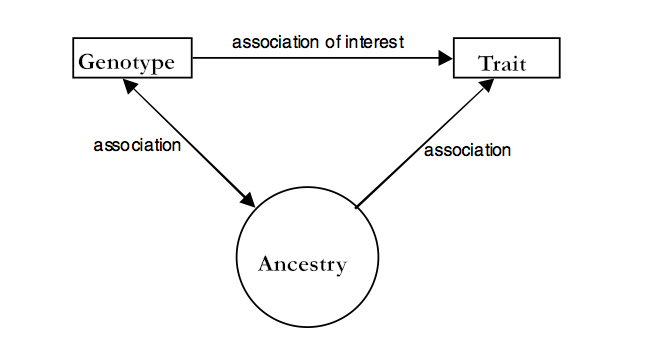
\includegraphics[scale=.4]{Figures/Confounding.png}
\end{figure}
In statistics, a {\bf confounding variable}  is an extraneous variable in a statistical model that correlates with both the dependent variable and the independent variable. 

\end{frame}



\begin{frame}
\frametitle{\bf Confounding due to Ancestry }
\begin{figure}
\centering
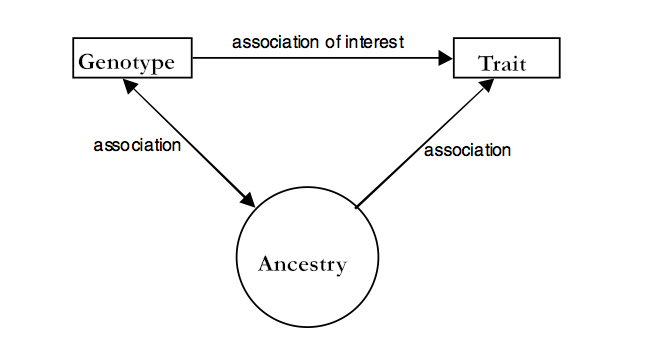
\includegraphics[scale=.4]{Figures/Confounding.png}
\end{figure}
\vspace{-.4cm}
\begin{itemize}
\item Ethnic groups (and subgroups) often share distinct dietary habits and other lifestyle characteristics that
leads to many traits of interest being correlated with ancestry and/or ethnicity.
\end{itemize}
\end{frame}


\begin{frame}
	\frametitle{Spurious Association}
	\begin{itemize}
		\item  Association test aims to compare of allele frequency between cases and controls.
		\item Consider a sample from 2 populations:  
\begin{minipage}{.55\textwidth}
	\begin{itemize}
		\item No differences in allele frequencies between cases/controls \textbf{within each population}
		\item Large differences in allele frequencies \textbf{between  populations}
		\item \textcolor{red}{Population 2} is overrepresented among cases in the sample.
		\newline $\implies$ spurious association between disease and genetic marker 
	\end{itemize}
\end{minipage}% This must go next to `\end{minipage}`
\begin{minipage}{.5\textwidth}
\begin{figure}
	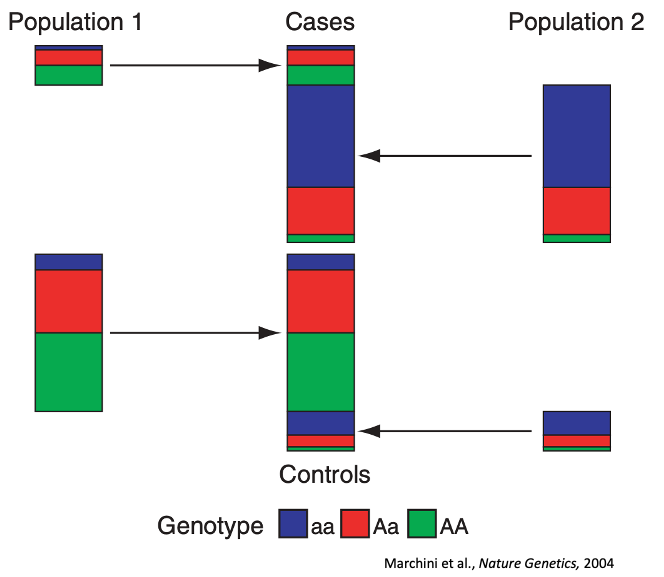
\includegraphics[scale=.25]{Figures/spurious_cc}
\end{figure}
\end{minipage}

		\end{itemize}
\end{frame}



\begin{frame}
\frametitle{\bf Genomic Control}
\begin{itemize}
\item Devlin and Roeder (1999) proposed correcting for substructure via a method called "genomic control."
\item If there is no population structure, then \textbf{at unlinked variants} the test statistic $T\sim \chi^{2}_1$ . \item   If there is population structure, the statistic will deviate from a $\chi^{2}_1$ distribution by an approximate constant factor  $T\sim \lambda\chi^{2}_1$ which is estimated as $$\lambda=\frac{median(T)}{median(\chi^{2}_1)}=\frac{median(T)}{.456}$$
\item    It is then applied to the test statistic values at all markers:
\[ \tilde{T}_j=\frac{T_j}{\lambda}\]
\end{itemize}
\end{frame}

\begin{frame}
	\frametitle{\bf Genomic Control}
\begin{figure}
	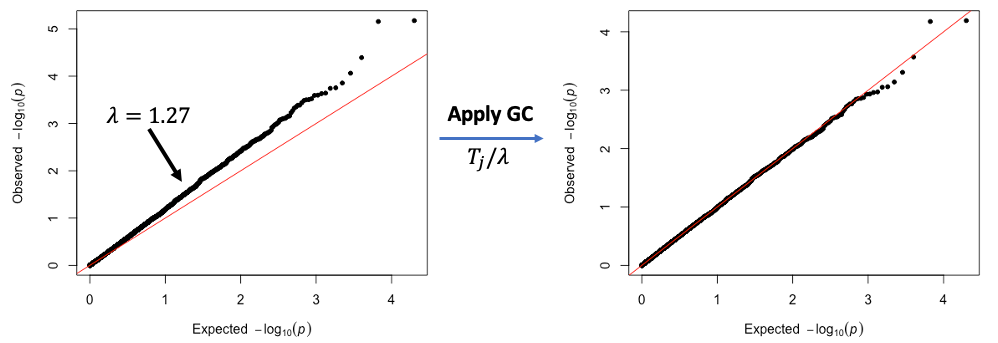
\includegraphics[scale=.4]{Figures/lgc_ex}
\end{figure}
\end{frame}


\begin{frame}
	\frametitle{\bf LD Score Regression}
	\begin{itemize}
		\item In practice,  $\lambda$ is computed using all variants
		\item Polygenicity can cause $\lambda > 1$
		\begin{itemize}
			\item Hard to separate confounding from polygenicity when $\lambda > 1$
		\end{itemize}
		\item LD score regression separates these by regressing "LD scores" $L_j$ on the test statistics
		$$ E[T_j] = {\color{red} Nh^2_g/M }\cdot L_j + {\color{blue} Na + 1} $$
		\textcolor{red}{Slope} $\rightarrow $ captures polygenicity\\
	\textcolor{blue}{Intecept} $\rightarrow $ captures confounding
	\end{itemize}
\end{frame}

\begin{frame}
	\frametitle{\bf LD Score Regression}
	\vspace{-1em}
\begin{figure}
	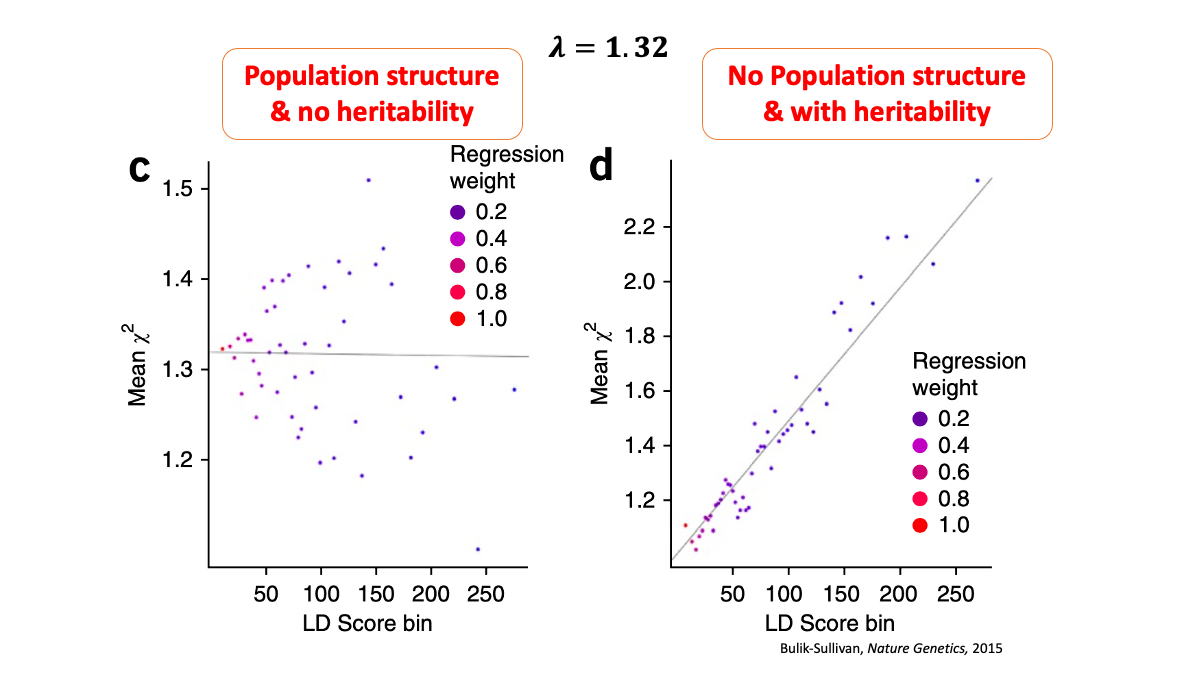
\includegraphics[scale=.35]{Figures/ldsc}
\end{figure}

\end{frame}



\begin{frame}
\frametitle{\bf Correcting for  Population Structure with PCA}
\begin{itemize}
\item Principal Components Analysis (PCA) is the most widely used approach for identifying and adjusting for ancestry differences among sample individuals
\item Consider the genetic relationship matrix  $\mathbf{\hat{\Psi}}$ discussed in the previous lecture with components $\hat{\psi}_{ij}$ for each pair of individuals as:
\[ \hat{\psi}_{ij}=\frac{1}{M}\sum_{l=1}^{M}\frac{(G_{il}-2\hat{p}_l)(X_{jl}-2\hat{p}_l)}{\hat{p}_l(1-\hat{p}_l)} \]
where $G_{il}=\{0,1,2\} $ is the genotype value and $\hat{p}_l$ is a corresponding allele frequency estimate at marker $l$
\end{itemize}
\end{frame}

\begin{frame}
\frametitle{\bf Correcting for  Population Structure with PCA}
\begin{itemize}
\item Price et al. (2006) proposed correcting for structure in genetic association studies by applying PCA to $\mathbf{\hat{\Psi}}$.
\item They developed a method called EIGENSTRAT for association testing in structured populations where the top principal components (highest eigenvalues)  are used as covariates in a linear regression model to correct for sample structure.

  \[ Y = \beta _0 + \beta _1G +\beta_2PC_1 +\beta_3PC_2 +\beta_4PC_3+ \cdots + \epsilon \]
  \[H_0: \beta _1=0 \text{ vs } H_a: \beta _1\ne0 \]
\end{itemize}
\end{frame}




\begin{frame}
\frametitle{\bf  Samples with Population Structure and Relatedness}
\begin{itemize}
\item Relatedness (family structure or cryptic relatedness) in the sample can lead to spurious association in genetic association studies 
\item The EIGENSTRAT method was developed for unrelated samples with population structure 
\begin{itemize}
	\item In the presence of relatedness, PCs may not fully capture this finer-scale structure
\end{itemize}
\item Many genetic studies include relatedness \& modeling it directly can lead to improvements in statistical power
\end{itemize}
\end{frame}


\section{Linear Mixed Models}


\begin{frame}
\frametitle{\bf Association Testing in Samples with Population Structure and Relatedness}
\vspace{-5pt}
\begin{itemize}
\item Linear mixed models (LMMs) have been demonstrated to be a flexible approach for association testing  in structured samples.  Consider the following model:
\end{itemize}
\begin{equation*}
\mathbf{Y}= {\color{red} \mathbf{X}\boldsymbol{\beta} + \mathbf{G_s}\gamma} +  \bg  + \bepsilon 
\end{equation*}

\begin{itemize}
\item {\bf Fixed effects:}
\begin{itemize}
\item  $\mathbf{X}$ is a $n \times (k+1)$ matrix of covariates that includes an intercept 
\item $\boldsymbol{\beta}$ is the $(k+1)$-length  vector of covariate effects
\item  $\gamma$ is the (scalar) association parameter of interest, measuring the effect of genotype on phenotype
\end{itemize}
\end{itemize}
\end{frame}



\begin{frame}
\frametitle{\bf Linear Mixed Models for Genetic Association}
\vspace{-5pt}
\begin{equation*}
\mathbf{Y}= \mathbf{X}\boldsymbol{\beta} + \mathbf{G_s}\gamma +  {\color{red}\bg  + \bepsilon }
\end{equation*}

\begin{itemize}
\item {\bf Random effects:}
\begin{itemize}
\item $\bg$ is a $n$-length vector of polygenic effects with  $\mathbf{g} \sim N(\mathbf{0},\sigma_g^2 \mathbf{\Psi})$
\begin{itemize}
\item   $\sigma^2_{g}$ represents additive genetic variance and $\mathbf{\Psi}$  is a $n\times n$ matrix of pairwise measures of genetic relatedness  (e.g. kinship matrix, GRM)
\item \textbf{g }should capture correlation between individuals due to genetic relatedness
\end{itemize}
\item $\boldsymbol{\epsilon}$ is a $n$-length vector with $ \boldsymbol\epsilon \sim N(\mathbf{0},\sigma_e^2 \mathbf{I})$
\begin{itemize}
\item $\sigma^2_{e}$  represents variance due to non-genetic effects assumed to be acting independently on individuals
\end{itemize}
\end{itemize}
\end{itemize}
\end{frame}


\begin{frame}
	\frametitle{\bf LMM methods for Quantitative Traits }
	\vspace{-2em}
	\begin{figure}
		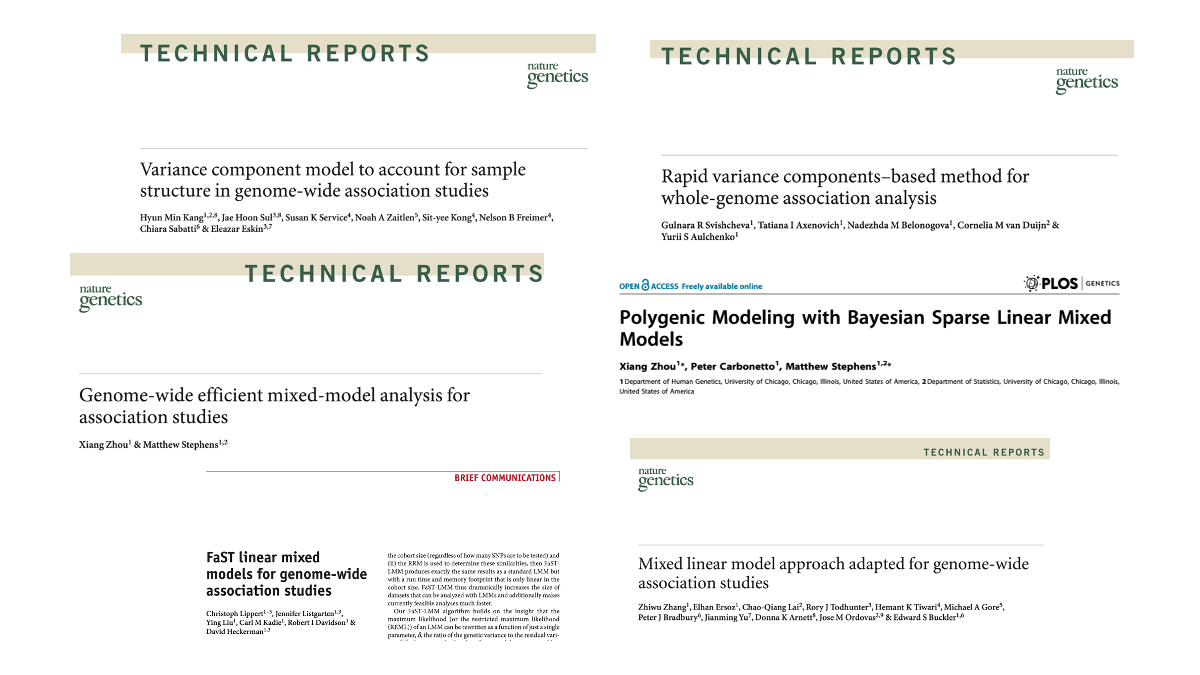
\includegraphics[scale=.35]{Figures/plots_lmm}
	\end{figure}
\end{frame}



\begin{frame}
\frametitle{\bf  LMMs: Two Step Procedure }
\begin{itemize}
\item Many LMM methods use a two-step procedure for GWAS
\item Step 1 considers a null model without the tested SNP of interest (i.e. $\gamma = 0$)
$$ \mathbf{Y}= \mathbf{X}\boldsymbol{\beta} +  \bg  + \bepsilon  $$
\begin{itemize}
	\item Obtain parameter estimates to get predictions for the polygenic effects \textbf{g}
\item  Same for all variants tested so only performed once which reduces the computational burden
\end{itemize}
\end{itemize}
\end{frame}



\begin{frame}
\frametitle{\bf  LMMs: Two Step Procedure }
\begin{itemize}
\item In Step 2, association testing of SNP and phenotype ($H_0:\gamma=0$)  is performed based on the model including the tested SNP
$$ \mathbf{Y}= \mathbf{X}\boldsymbol{\beta} + \mathbf{G_s}\gamma +  \bg  + \bepsilon $$
\item A score test is performed using the null parameter estimates obtained from Step 1.
\item Use Leave-One-Chromosome-Out (LOCO) scheme in Step 1 so polygenic term doesn't capture effects on tested chromosome (i.e. proximal contamination)
\end{itemize}
\end{frame}

\begin{frame}
	\frametitle{\bf  LMMs: Two Step Procedure }
	\begin{itemize}
		\item Many methods differ mainly in  Step 1 approach
		\begin{itemize}
			\item Model used for the additive polygenic random effect term
			\begin{figure}
				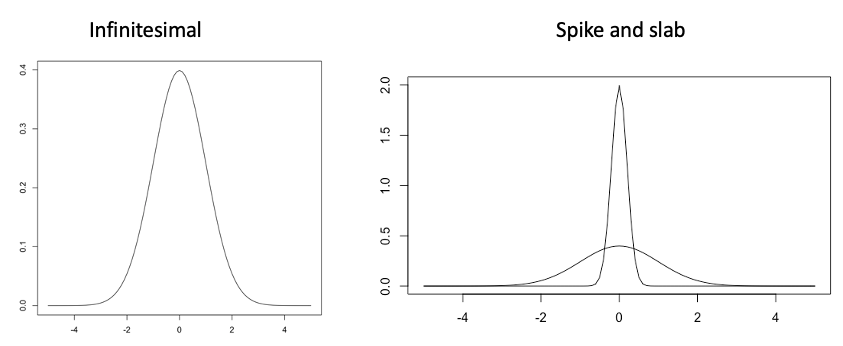
\includegraphics[scale=.3]{Figures/lmm_priors}
			\end{figure}
			\item Algorithm used to obtain parameter estimates
			\begin{itemize}
				\item  Parameter estimates are obtained using various approaches (e.g. maximum likelihood,  restricted maximum likelihood [REML],...) 
			\end{itemize}
		\end{itemize}
	\end{itemize}
\end{frame}




\begin{frame}
	\frametitle{\bf  LMMs on biobank scale data }
	\begin{itemize}
		\item Largest biobanks have gathered data on 100,000s of individuals (e.g. UK Biobank at $N=500,000$ individuals)
		\item Many LMM methods involved computationally expensive operations due to the $N\times N$ GRM
		\begin{figure}
			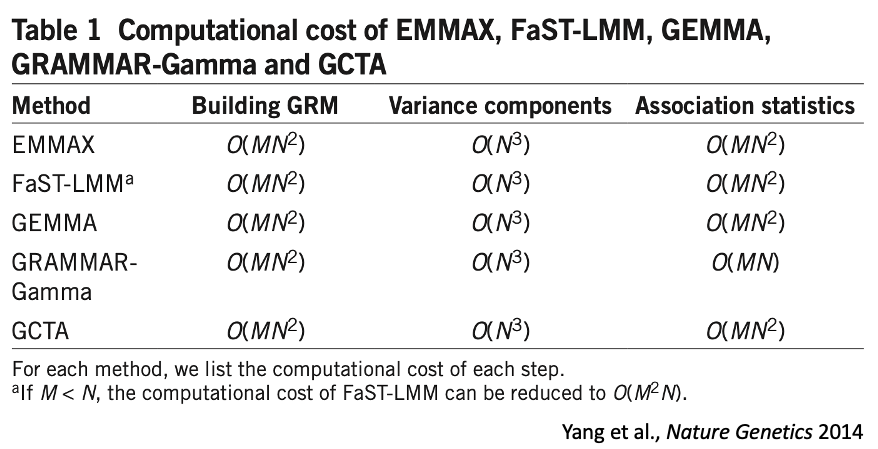
\includegraphics[scale=.3]{Figures/lmm_cost}
		\end{figure}
	\end{itemize}
\end{frame}

\begin{frame}
	\frametitle{\bf  LMMs on biobank scale data }
	
	\begin{minipage}{.7\textwidth}
	\begin{itemize}
	\item Loh et al. (2015) proposed BOLT-LMM which used very efficient algorithms  (Variational Bayes) to reduce scaling to $\sim O(MN^{1.5})$ for Step 1 and could be applied to biobank-scale data
	\item Jiang et al. (2019) proposed fastGWA which made use of a sparse GRM leading to further improvements for Step 1 $\sim O(MN)$ 
\end{itemize}
	\end{minipage}% This must go next to `\end{minipage}`
	\begin{minipage}{.3\textwidth}
	\begin{figure}
	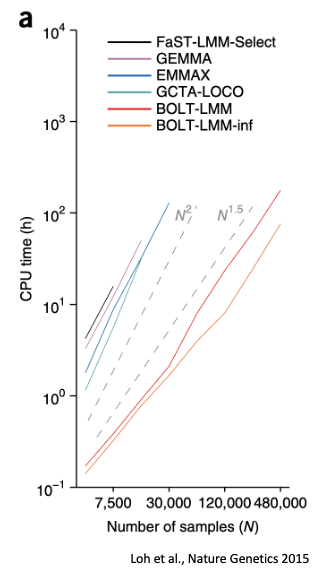
\includegraphics[scale=.4]{Figures/lmm_bolt}
\end{figure}
	\end{minipage}

\end{frame}

\section{Whole Genome Regression}
\begin{frame}
	\frametitle{\bf  LMMs \&  Whole Genome Regression}
	\begin{itemize}
		\item LMMs are closely related to whole genome regression
	\end{itemize}
\vspace{-1em}
	\begin{figure}
	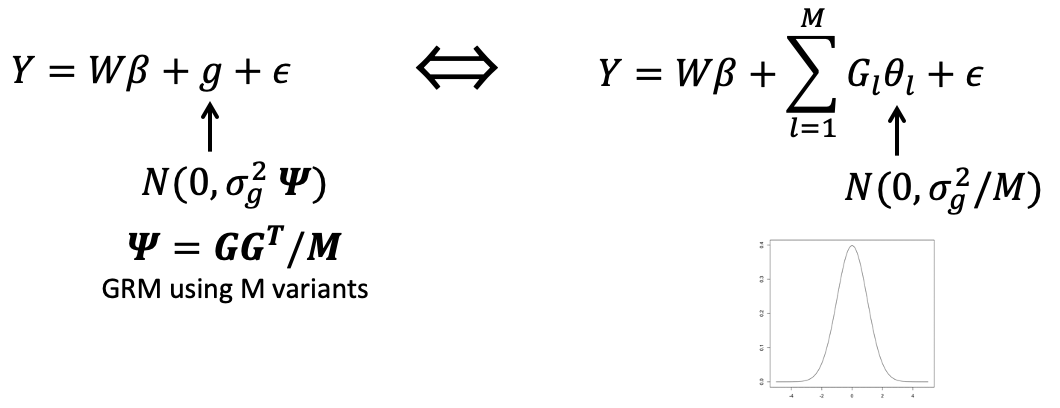
\includegraphics[scale=.4]{Figures/lmm_wgr}
\end{figure}
\end{frame}

\begin{frame}
	\frametitle{\bf  LMMs \&  Whole Genome Regression}
	\begin{itemize}
		\item LMMs are closely related to whole genome regression
	\end{itemize}
	\vspace{-1em}
	\begin{figure}
		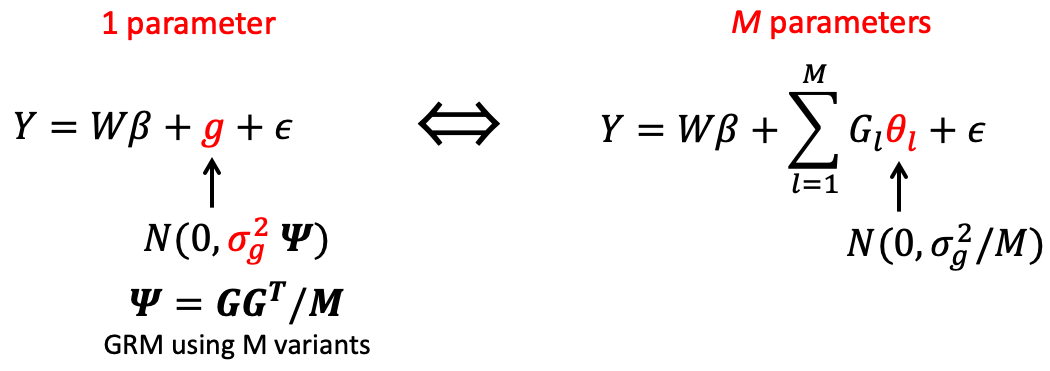
\includegraphics[scale=.4]{Figures/lmm_wgr2}
	\end{figure}
\end{frame}


\begin{frame}
	\frametitle{\bf  REGENIE: Whole Genome Regression}
	\begin{itemize}
		\item Step 1: computationally efficient whole genome regression
		$$ \mathbf{Y}= \mathbf{X}\boldsymbol{\beta} +  \sum_{l=1}^MG_l\theta_l + \bepsilon  $$
		\item M is usually $\sim$ 500,000 SNPs across the genome
		\item REGENIE splits genetic data into blocks and run local regressions in each block to reduce computational burden
	\end{itemize}
\end{frame}


\begin{frame}
	\frametitle{\bf  REGENIE: Whole Genome Regression}
	\vspace{-1em}
\begin{figure}
	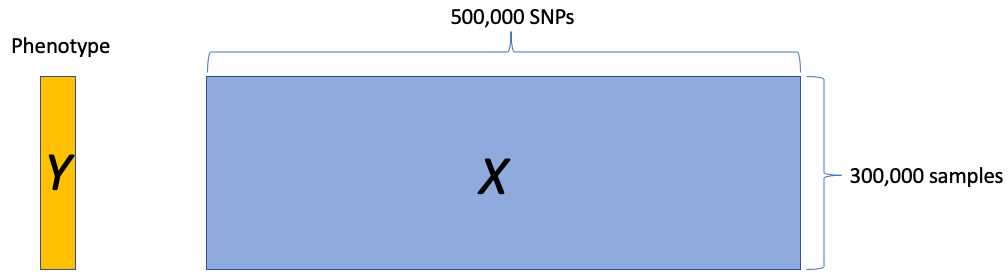
\includegraphics[scale=.35]{Figures/regenie_wgr}
\end{figure}
\end{frame}

\begin{frame}
	\frametitle{\bf  REGENIE: Whole Genome Regression}
	\vspace{-1em}
	\begin{figure}
		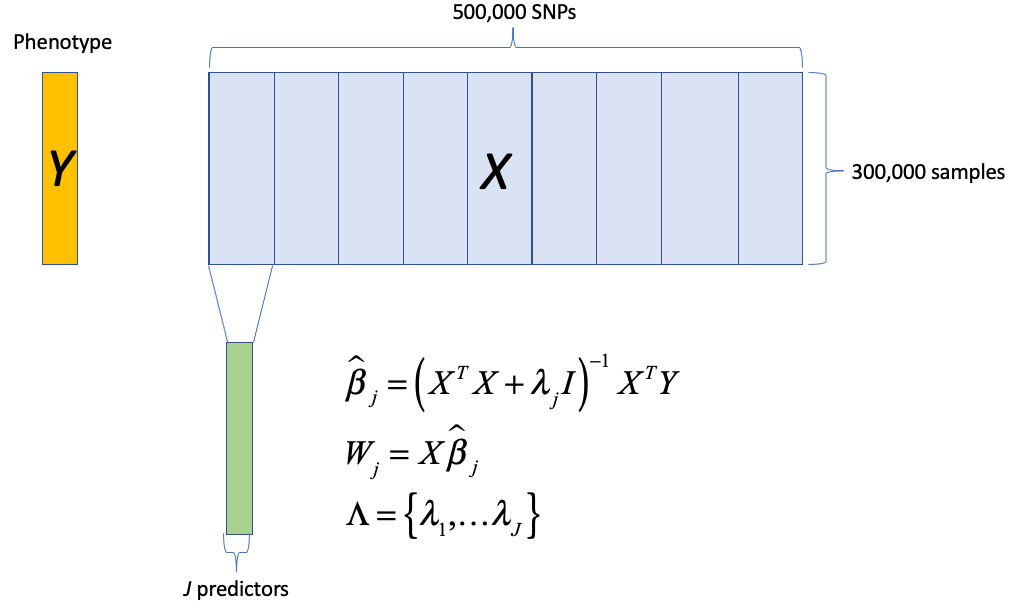
\includegraphics[scale=.35]{Figures/regenie_wgr2}
	\end{figure}
\end{frame}

\begin{frame}
	\frametitle{\bf  REGENIE: Whole Genome Regression}
	\vspace{-1em}
	\begin{figure}
		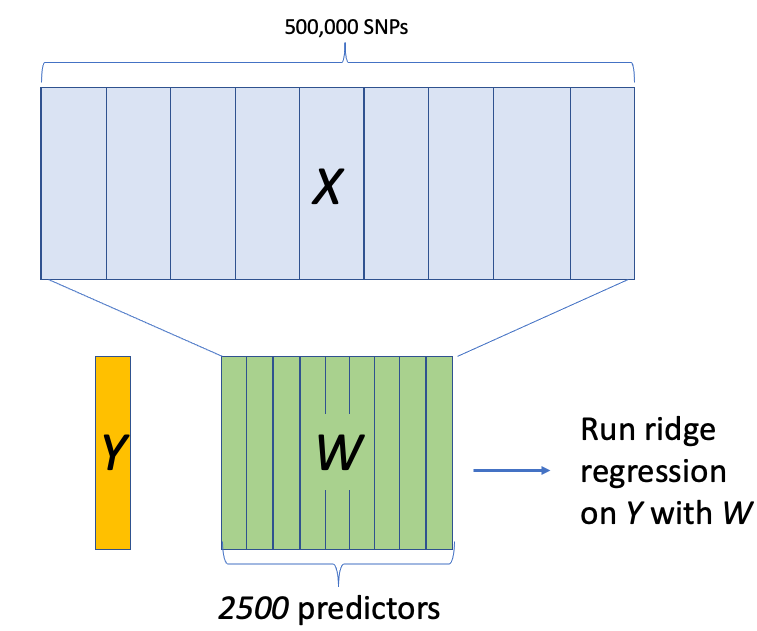
\includegraphics[scale=.35]{Figures/regenie_wgr3}
	\end{figure}
\end{frame}

\begin{frame}
	\frametitle{\bf  REGENIE: Whole Genome Regression}
	\begin{itemize}
		\item Step 1: computationally efficient whole genome regression
		$$ \mathbf{Y}= \mathbf{X}\boldsymbol{\beta} +  \sum_{l=1}^MG_l\theta_l + \bepsilon  $$
		\item Divide into two levels of regressions
		\begin{itemize}
			\item Reads genetic data in blocks and within each block fits ridge regression (penalized linear regression)
			\item Fit another round of ridge regression on all the block predictors
		\end{itemize}
		\item  Polygenic predictions ($\sum_{l=1}^MG_l\hat{\theta}_l $) capture population structre, relatedness as well as polygenicity
	\end{itemize}
\end{frame}


\begin{frame}
	\frametitle{\bf  REGENIE: Whole Genome Regression}
	\begin{itemize}
		\item Step 2:  test the association parameter $\gamma$ under the null hypothesis of $H_0: \gamma=0.$
		$$ \mathbf{Y}= \mathbf{X}\boldsymbol{\beta} + G_s\gamma+ \sum_{l=1}^MG_l\hat\theta_l + \bepsilon  $$
		\item Test on millions of genetic variants (imputed or whole exome)
		\item Also works on binary traits where logistic regression is used instead of linear regression
		\end{itemize}
\centering\url{https://rgcgithub.github.io/regenie/}
\end{frame}


\section{References}


\begin{frame}
\frametitle{\bf References}
\begin{itemize}

\item  Devlin, B. \& Roeder, K. Genomic Control for Association Studies. \textit{Biometrics} \textbf{55}, 997-1004 (1999).
\item Bulik-Sullivan, B.K. et al. LD Score regression distinguishes confounding from polygenicity in genome-wide association studies. \textit{Nature Genetics} \textbf{47}, 291-295 (2015).
\item Price, A.L. et al. Principal components analysis corrects for stratification in genome-wide association studies.\textit{ Nature Genetics} \textbf{38}, 904-909 (2006).
\item Yang, J., Zaitlen, N.A., Goddard, M.E., Visscher, P.M. \& Price, A.L. Advantages and pitfalls in the application of mixed-model association methods. \textit{Nature Genetics} \textbf{46}, 100-106 (2014).

\end{itemize}

\end{frame}

\begin{frame}
\frametitle{\bf References}

\begin{itemize}

\item Loh, P.-R. et al. Efficient Bayesian mixed-model analysis increases association power in large cohorts.\textit{ Nature Genetics} \textbf{47}, 284-290 (2015).
\item Jiang, L. et al. A resource-efficient tool for mixed model association analysis of large-scale data. \textit{Nature Genetics} \textbf{51}, 1749-1755 (2019).
\item Zhou, W. et al. Efficiently controlling for case-control imbalance and sample relatedness in large-scale genetic association studies. \textit{Nature Genetics} \textbf{50}, 1335-1341 (2018).
\item Mbatchou, J. et al. Computationally efficient whole-genome regression for quantitative and binary traits. \textit{Nature Genetics} \textbf{53}, 1097-1103 (2021).
\end{itemize}


\end{frame}


\end{document}
